\documentclass{standalone}
\usepackage{ tikz }
\usepackage{ xparse }
\usepackage{../../../macros}

\begin{document}
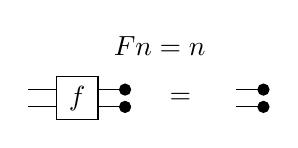
\begin{tikzpicture}[yscale=-1,x=1em,y=1.25em]

    \draw (0.5,-0.25) -- (1.5,-0.25);
    \draw (0.5,0.25) -- (1.5,0.25);
    \node[draw, minimum height = 1.5em, minimum width = 1.5em, anchor = west] at (1.5,0){$f$};
    \draw (3,-0.25) -- (4,-0.25);
    \draw (3,0.25) -- (4,0.25);
    \filldraw (4,-0.25) circle (2pt);
    \filldraw (4,0.25) circle (2pt);

    \node at (6,0) {$=$};
    \node at (5.25,-1.5) {$F \seq \cdel{n} = \cdel{n}$};

    \draw (8,-0.25) -- (9,-0.25);
    \filldraw (9,-0.25) circle (2pt);
    \draw (8,0.25) -- (9,0.25);
    \filldraw (9,0.25) circle (2pt);

\end{tikzpicture}
\end{document}